\documentclass{utue} %uumi.cls required for Uni Ulm corporate design
\usepackage{listings}
\usepackage{caption}
\usepackage{geometry}
\usepackage{url}
\usepackage{amssymb}
\usepackage{mathrsfs}
\usepackage{tikz}
\usepackage{subcaption}

\lstset{
basicstyle=\rmfamily,
columns=fullflexible,
frame=tb,
framexleftmargin=20pt,
captionpos=t,
breaklines=true,
mathescape,
numbers=left,
numberstyle=\small,
numbersep=5pt,
xleftmargin=20pt,
tabsize=3,
escapeinside={\{}{\}},
keywords={Input, Output, if, else, then, return, for, all, do}
}
\DeclareCaptionFormat{listing}{\hrule#1#2#3}
\captionsetup[lstlisting]{format=listing,singlelinecheck=false, margin=0pt,labelsep=space,labelfont=bf}
\renewcommand*\thelstnumber{\arabic{lstnumber}:}

% Values for title generation
\title{Dual tree traversal for nearest neighbour search}
\author{Fabian Fritz}
\date{\today}

% Subtitle is optional. It represents what kind of work you did.
\subtitle{Praktikum Computergrafik SoSe2016}

\begin{document}

% You can place a teaser as follows. (Otherwise, just uncomment the following part)
\teaser{
    
\includegraphics[width=\textwidth]{images/teaser.jpg}
    \caption{You can place a teaser here.}
    \label{fig:teaser}
}     

% Creates title of document and additional title page.
\maketitle

\section*{Abstract}

Give an overview over your project here. Give a glimpse insight in the problem and write why it is important to be solved. Write what you did to make your implementation better than the state of the art implementations.


\section{Introduction}

Aligning two sets of points in multiple dimensions (known as point set registration or point matching) is an important step if one is interested in comparing two point clouds.
These points might originate from an accurate 3d model of an object, a 3d scan or from other tools to acquire multidimensional data. Even if the same method was used for both sets, the number of points and their exact positions might differ. Also, in case the two sets actually have the same number of points, one cannot assume the points appear in the same order. Let $\mathbf{Q},\mathbf{P}$ be two point sets, $\mathbf{q} \in \mathbf{Q}, \mathbf{p} \in \mathbf{P}$ be points in the respective set. To align the two sets, it is necessary then to find a transformation$$
\min \sum_{i,j}^{|P|,|Q|} |\mathbf{p_i}-\mathcal{T}(\mathbf{q_j})|
$$
where $\mathcal{T}(\mathbf{Q}) = s\mathbf{R}\mathbf{Q} + \mathbf{t}$ is a rigid transformation of set $\mathbf{Q}$ with $s$ being the scaling factor, $\mathbf{R}$ being a rotation matrix and $\mathbf{t}$ being a translation vector. This is also known as a Procrustes transformation.

\subsection{Iterative closest point algorithm}
The iterative-closest-point (ICP) algorithm solves both problems: finding the best corespondence between the sets of points and aligning the point clouds according to this. To do this, it is necessary first to find the nearest neighbor for each point. Then, the sets of points can be aligned by minimizing the total distance between the points. These two steps are repeated until either the point clouds are perfectly aligned or the total distance is below some specified threshold.

While the second step, minimizing the distances between points, can be trivially implemented, e. g. by using the least squares method, there are multiple ways of implementing and optimizing the nearest neighbor search (NNS). One way of improving the performance of an NNS is by using dedicated data structures, such as trees, for either one or both sets of points.
\subsection{k-d trees and dual traversal}
Both Besl et. al. and McKay as well as Simon recommend k-d trees to accelerate the search \cite{icp,simon1996fast}. For NNS this space-partitioning structure allows to efficiently remove, or prune whole sets of points that are irrelevant for the search. To build a kdtree, the steps are:
\begin{enumerate}
\item For a given dimension, find the median point with regards to that dimension
\item Add a node to the tree and associate it with the found point
\item Recurse into the point sets right and left of the median element and add them as leaves to the current node
\end{enumerate}
During the recursion all dimension are being cycled through. The process of building a k-d tree can be shown to have complexity $O(n \log n)$. Notice that this algorithm is inherently recursive and therefore sequential.

While using a kdtree for one set of the points is quite intuitive, the method of using treelike structures for both sets was proposed later and is known as dual-tree traversal \cite{firstdual}.\\


There is a large variety of trees one can use in conjunction with the dual tree traversal algorithm, and their influence on the performance has already been studied comprehensively. However, little was done to investigate how to run this algorithm in parallel. In particular, the possibility of utilizing the graphics processing unit(GPU) as a means of computation for this search hasn't been explored thoroughly.

With this work we want to advance Curtis' work \cite{improving} towards a parallel implementation of this general approach. By comparing the performance of a brute-force approach and search on a single kdtree and search on two R-trees, both as sequential and parallel implementations, we want to show how these data structures influence the runtime and why there are difficulties in bringing the optimal version of this algorithm to the GPU is non-trivial.
\section{Related Work} 

The ICP algorithm already was described in 1992 by Besl et. al.\cite{icp}. Since then, many optimizations have been proposed, both in terms of matching quality and speed \cite{comparison}. In particular, the k-d tree was proposed early as an improvement for the performance of the algorithm \cite{simon1996fast}.

Curtin describes a framework on how to implement dual tree traversal, independent of the choice of the tree or the particular search problem\cite{improving}. His algorithm in each step processes two nodes $\mathscr{N}_q,\mathscr{N}_r$ from the respective trees. If the algorithm reaches the leaf nodes and detects a smaller neighbor, this candidate is stored in an array $N$ and its distance in $D$ (see listing \ref{basecase}).

\begin{figure}
	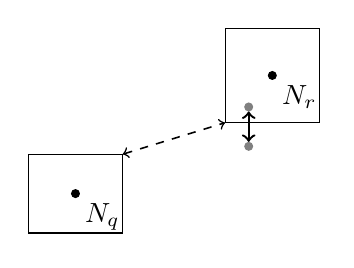
\begin{tikzpicture}
		\draw (0.2,0.2) rectangle (1.4,1.2) node[pos=.5,circle,draw=black,fill=black,inner sep=1pt] (nodeanchor) {};
		\node[below right] at (nodeanchor) {$N_q$};
		\node[circle,draw=gray,fill=gray,inner sep=1pt] at (3,1.8) (child1) {};
		\node[circle,draw=gray,fill=gray,inner sep=1pt] at (3,1.3) (child2) {};
		\draw[<->,line width=0.3mm] (child1) -- (child2);
		\draw (2.7,1.6) rectangle (3.9,2.8) node[pos=.5,circle,draw=black,fill=black,inner sep=1pt] (nodeanchor2) {};
		\draw[<->,line width=0.2mm,dashed] (1.4,1.2) -- (2.7,1.6);
		\node[below right] at (nodeanchor2) {$N_r$};
	\end{tikzpicture}
	\caption{Pruning in dual traversal: this pair of nodes would not be processed as the maximal distance of a descendant in $N_r$ (indicated as gray dot) is already smaller than anything within the bounds of $N_q$.}
	\label{fig:pruning}
\end{figure}
\begin{lstlisting}[caption={Simple \texttt{BaseCase()} for nearest neighbor search.},label=basecase]
Input: query point $p_q$, reference point $p_r$, candidate point $N[p_q]$, candidate distance $D[p_q]$
Output: distance $d(p_q,p_r)$
if $d(p_q,p_r) < D[p_q]$ then
	$N[p_q] \leftarrow p_r$
	$D[p_q] \leftarrow d(p_q, p_r)$
\end{lstlisting}
One important aspect with tree-based searches is pruning. Curtin recommends to have some boundary information within the nodes. Then, the minimal distance between the boundaries $d_{min}(\mathscr{N}_q,\mathscr{N}_r)$ can be compared to the distance of the descendant $p \in \mathscr{D}^p$ with the largest distance $max_{p \in \mathscr{D}^p(\mathscr{N}_q)}D_{p_q}$. If the distance between boundaries is larger, this pair of nodes can be dismissed (see also figure \ref{fig:pruning}).

The trivial version of Curtins algorithm has two parts: the traversal function with pruning and the basecase function (see listing \ref{dual}).
\begin{lstlisting}[caption={\texttt{DualTraversal}($\mathscr{N}_q,\mathscr{N}_r$)},label=dual]
Input: query node $\mathscr{N}_q$, reference node $\mathscr{N}_r$
{\{Calculate bound and prune if possible.\}}
$\{\mathscr{D}^p(\mathscr{N}_q)$ represents the set of descendant points of the query node $\mathscr{N}_q$}
$b\leftarrow \max_{p \in \mathscr{D}^p(\mathscr{N}_q)}D_{p_q}$
if $d_{min}(\mathscr{N}_q, \mathscr{N}_r) > b$ then
	return
if $\mathscr{N}_q$ and $\mathscr{N}_r$ are both leaves then
	BaseCase($p_q$, $p_r$)
else if $\mathscr{N}_q$ is a leaf and $\mathscr{N}_r$ is not then
	DualTraversal($\mathscr{N}_q, \mathscr{N}_{p-leftchild}$)
	DualTraversal($\mathscr{N}_q, \mathscr{N}_{p-rightchild}$)
else if $\mathscr{N}_q$ is not a leaf and $\mathscr{N}_r$ is one then
	{\{Handle case accordingly...\}}
else if both $\mathscr{N}_q$ and $\mathscr{N}_r$ have children then
	{\{Handle case accordingly...\}}
\end{lstlisting}

The author then proposes an improvement: instead of using the comparison described above only for pruning, this can also be used as a value for prioritization. This is therefore extracted in a third part: the score function (see listing \ref{score}).
\begin{figure}[h]
\begin{lstlisting}[caption={Simple \texttt{Score()} for nearest neighbor search},label=score]
Input: query node $\mathscr{N}_q$, reference node $\mathscr{N}_r$
Output: a score for the node combination $(\mathscr{N}_q, \mathscr{N}_r)$ or $\infty$ if it should be pruned
if $d_{min}(\mathscr{N}_q, \mathscr{N}_r) > B_{df}(\mathscr{N}_q)$ then
	return $\infty$
return $d_{min}(\mathscr{N}_q, \mathscr{N}_r)$
\end{lstlisting}
\end{figure}
Equipped with these three parts, a priority queue is used to handle the processing order of the node pairs. Curtin shows that with this version a significant speedup can be achieved (see listing \ref{priorized}).
\begin{figure}[h]
\begin{lstlisting}[caption={\texttt{ImprovedDualTraversal}($\mathscr{N}_q,\mathscr{N}_r$)},label=priorized]
Input: query node $\mathscr{N}_q$, reference node $\mathscr{N}_r$
Output: none
if $\mathscr{N}_q$ and $\mathscr{N}_r$ are both leaves then
	BaseCase($p_q$, $p_r$)
else if $\mathscr{N}_q$ is a leaf and $\mathscr{N}_r$ is not then
	$s \leftarrow$ Score($\mathscr{N_q}$, $\mathscr{N}_{r-leftchild}$)
	if $s < \infty$ then
		push $(\mathscr{N}_q, \mathscr{N}_r)$ into $q$ with priority $1/s$
	$s \leftarrow$ Score($\mathscr{N_q}$, $\mathscr{N}_{r-rightchild}$)
	if $s < \infty$ then
		push $(\mathscr{N}_q, \mathscr{N}_r)$ into $q$ with priority $1/s$
else if $\mathscr{N}_q$ is not a leaf and $\mathscr{N}_r$ is one then
	{\{Handle case accordingly...\}}
else if both $\mathscr{N}_q$ and $\mathscr{N}_r$ have children then
	{\{Handle case accordingly...\}}
\end{lstlisting}
\end{figure}
\section{Methodology}
We implemented different algorithms to compare their performance at nearest neighbor search:
\begin{itemize}
\item brute force attempt (CPU)
\item k-d tree search (CPU)
\item k-d tree search (GPU)
\item dual tree search (CPU)
\item dual tree prioritized search (CPU)
\item dual tree search (GPU)
\end{itemize}
Since the brute force attempt, the k-d tree (CPU, GPU) and dual tree search are trivial or discussed elsewhere extensively, we will only discuss details about the dual tree search on GPU.

The first step was to find an appropriate tree structure. We chose R-trees, as k-d trees can easily be adapted to and they provide the boundary information that is necessary for pruning (see figure \ref{rtree}). Each node has a rectangular boundary that encloses the minimal area to include all descendants \cite{rtree}. For consistency, even leaf nodes have this kind of information, only that their area is infinitesimal. Notice however that after doing a transformation this tree might becomes invalid and needs to be rebuild in each step of the ICP algorithm. As a remedy for this problem, a ball tree could be used instead, as it will maintain validity. This variant however is also more complicated to build \cite{balltree}.

Since the GPU isn't well suited for a recursive algorithm, we had to find a way of quickly occupying as many threads as possible. A queue-like array that stores the items that are to be processed allows a subsequent parallel algorithm to both access and write many items at the same time. So instead of recursively calling the traversal function again (as in listing \ref{dual}, line 10,11,...),
\begin{figure}[h]
	\begin{subfigure}{.24\textwidth}
		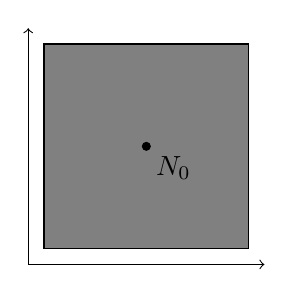
\begin{tikzpicture}
		\draw[->] (0,0) -- (0,3);
		\draw[->] (0,0) -- (3,0);
		\draw[fill=gray] (0.2,0.2) rectangle (2.8,2.8) node[pos=.5,circle,draw=black,fill=black,inner sep=1pt] (nodeanchor) {};
		\node[below right] at (nodeanchor) {$N_0$};
		\end{tikzpicture}
	\end{subfigure}
	\begin{subfigure}{.24\textwidth}
	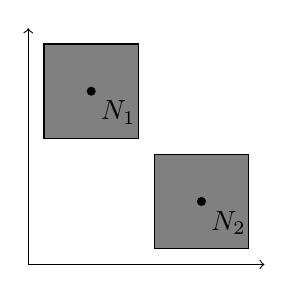
\begin{tikzpicture}
		\draw[->] (0,0) -- (0,3);
		\draw[->] (0,0) -- (3,0);
		\draw[fill=gray] (0.2,1.6) rectangle (1.4,2.8) node[pos=.5,circle,draw=black,fill=black,inner sep=1pt] (nodeanchor) {};
		\draw[fill=gray] (1.6,0.2) rectangle (2.8,1.4) node[pos=.5,circle,draw=black,fill=black,inner sep=1pt] (nodeanchor2) {};
		\node[below right] at (nodeanchor) {$N_1$};
		\node[below right] at (nodeanchor2) {$N_2$};
	\end{tikzpicture}
	\end{subfigure}
	\caption{R-tree at root level and the level below.}
	\label{rtree}
\end{figure}


\section{Evaluation}

\section{Conclusion \& Outlook}
We have implemented and compared different methods of nearest neighbor search for usage with the ICP algorithm. In particular, we were interested in bringing Curtins approach\cite{improving} of dual tree traversal to the GPU.

On the CPU, prioritizing the traversal brings a significant speedup for a sufficient number of node pairs. This variant however proved difficult to implement for the GPU, since by its very nature it relies on a sequential way of processing the pairs in order to prune unnecessary work.

Further work is needed in order to introduce prioritization to a parallel dual tree traversal.

\bibliographystyle{alpha}
\bibliography{bibliography}

\end{document}

